\documentclass[12pt,a4paper]{report}
\usepackage[utf8]{inputenc}
\usepackage[portuguese]{babel}
\usepackage[T1]{fontenc}
\usepackage{amsmath}
\usepackage{amsfonts}
\usepackage{amssymb}
\usepackage{graphicx}
\usepackage{fourier}
\usepackage[left=1.5cm,right=2cm,top=1.5cm,bottom=1.5cm]{geometry}
\author{Luiz Guilherme - Professor de Matemática}
\title{Matemática e Raciocínio Lógico\\ para Concursos Públicos}
\date{Última atualização:  \today \\ \qrcode{https://docs.google.com/viewer?url=https://raw.githubusercontent.com/lgfpcampos/Concursos/main/apostila.pdf}} 
\usepackage{tikz}
\usepackage{tcolorbox}
\usepackage{hyperref}
\usepackage{qrcode}
\usepackage{xcolor}
\usepackage{fontawesome}
\usepackage{enumerate}
\usepackage[Bjornstrup]{fncychap}
\usepackage{multicol}
\usepackage{makeidx}




\begin{document}

\newcommand{\quest}[4]{ \item 
	\textbf{#1} {\color{red}\faYoutubePlay}\\ % Banca e Concurso
	 {#2}\\ %enunciado
		\begin{minipage}{12cm}
		\begin{enumerate}
			{#3} %alternativas
		\end{enumerate}
	\end{minipage}
	\qrcode{#4&list=UULFeA_dOOqAA4DB92B_BWDU7Q}} %youtube


\maketitle
\tableofcontents	

\begin{enumerate}
\chapter{Análise Combinatória}

\quest{Técnico Interno BBTS 2023 - FGV}{No quadro abaixo, considere os caminhos que formam a palavra BRASIL começando em uma letra B e caminhando para a direita ou para baixo.
\begin{center}
\begin{tabular}{cccccc}
  &   &   &   &   & B \\ 
  &   &   &   & B & R \\ 
  &   &   & B & R & A \\ 
  &   & B & R & A & S \\ 
  & B & R & A & S & I \\ 
B & R & A & S & I & L \\ 
\end{tabular} 
\end{center}
Assinale a opção que indica o número total de caminhos diferentes.}{
\item 12.
\item 18.
\item 24.
\item 32
\item 64.}
{https://youtu.be/4iPSTxj3XdU}
\chapter{Conjuntos}
\quest{Oficial de Justiça 2023 - VUNESP}{Sobre um grupo de atletas sabe-se que 15 praticam
natação, atletismo e ciclismo, 20 praticam somente n­atação e atletismo, 27 praticam somente natação e
c­iclismo, e 25 praticam somente atletismo e ciclismo. Se 70 atletas desse grupo praticam natação, 61 praticam atletismo, e 75 praticam ciclismo, então é verdade que, das alternativas a seguir, a que contém a porcentagem que mais se aproxima da relação entre o número de atletas que praticam um único esporte o número total de atletas desse grupo é}
{\item 12\%
\item 18\%
\item 20\%
\item 16\%
\item 14\%
}{https://youtu.be/SYUNxu4fcF8}
\chapter{Estatística}

\section{Medidas de Tendência Central}

\quest{Oficial de Justiça 2023 - VUNESP}{O gráfico apresenta o número de acertos na prova de Língua Portuguesa e de Matemática, aplicada a dois candidatos, A e B, em um concurso interno para promoção de cargo:\\
	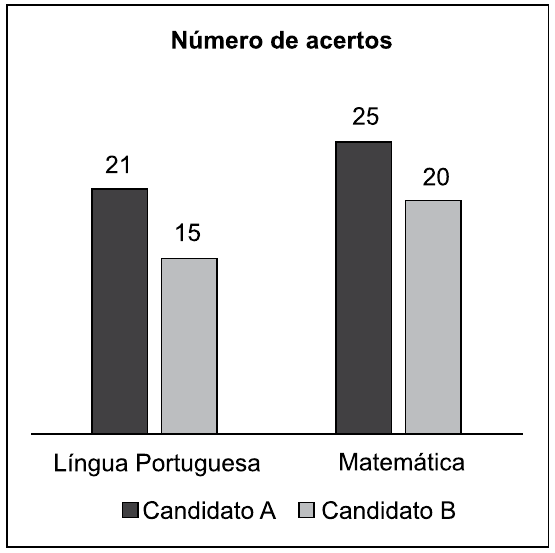
\includegraphics[scale=.5]{fig001.png}\\
Sabendo-se que a prova de Língua Portuguesa tinha 	peso 2 e a de Matemática tinha peso 3 para o cargo em 	concurso, que cada uma das provas tinha 50 questões, 	e que a nota de cada prova é igual ao número de acertos correspondente, é correto afirmar que o número de questões de Matemática que o candidato B deveria ter acertado a mais, para que a média aritmética ponderada das notas das suas provas fosse igual à média aritmética ponderada das notas das provas do candidato A, é igual a}
{\item 9.
\item 20.
\item 10.
\item 29.
\item 27.}
{https://youtu.be/BvsQZctqarQ}

\section{Medidas de Dispersão}

\quest{Transpetro 2023 - CESGRANRIO}
{Uma empresa, em reconhecimento ao desempenho de 10 de seus funcionários, decide dar-lhes um bônus. Para tanto, a empresa distribuiu um total de R\$ 25.000,00, de acordo com a Tabela a seguir:
\begin{center}
\begin{tabular}{c|c}
\hline 
Número de   & Valor do Bônus\\ 
funcionários & (em reais) \\ 
\hline
6 & 2000 \\ 
\hline 
2 & 2500 \\ 
\hline 
2 & 4000 \\ 
\hline 
\end{tabular} 
\end{center}
Nessas condições, o desvio padrão dos bônus pagos é dado por}
{
\item $\sqrt{\dfrac{36 \cdot 2000^2 + 4\cdot 2500^2 + 4\cdot 4000^2}{10}}$
\item $\sqrt{\dfrac{36 \cdot 500^2 + 4\cdot 2500^2 + 4\cdot 1500^2}{10}}$
\item $\sqrt{\dfrac{6 \cdot 2000^2 + 2\cdot 2500^2 + 2\cdot 4000^2}{10}}$
\item $\sqrt{\dfrac{500^2 + 1500^2}{10}}$
\item $\sqrt{\dfrac{6 \cdot 500^2 + 2\cdot 1500^2}{10}}$
}
{https://youtu.be/fDPDxc8zjzY}

\quest{Transpetro 2023 - CESGRANRIO}
{Em uma escola, há cinco turmas que fizeram uma prova de matemática, e cada uma possui 60 estudantes. As notas obtidas em cada turma tiveram as seguintes distribuições:
\begin{itemize}
\item Turma 1: 30 notas iguais a 0 e 30 notas iguais a 10;
\item Turma 2: 30 notas iguais a 2 e 30 notas iguais a 8;
\item Turma 3: 30 notas iguais a 3 e 30 notas iguais a 7;
\item Turma 4: 30 notas iguais a 4 e 30 notas iguais a 6;
\item Turma 5: 60 notas iguais a 5.
\end{itemize}
Em qual das turmas o desvio-padrão das notas obtidas foi igual a zero?}
{
\item Turma 1
\item Turma 2
\item Turma 3
\item Turma 4
\item Turma 5}
{https://youtu.be/KkKYd_ILgn8}
\chapter{Expressões Algébricas}

\quest{Técnico Interno BBTS 2023 - FGV}{Considere as seguintes operações com números racionais:\\
$x\#y = x^2 + y^2$\\
$x\&y = x - 2y$\\
O valor de $(3\#1)&(7\&2)$ é}{
\item −4.
\item −2.
\item 0.
\item 2.
\item 4.}
{https://youtu.be/vwhbHJj6Ey8}
\chapter{Função Afim}
\quest{Banco do Brasil 2023- CESGRANRIO}{Um fabricante sabe que o custo de produção de 1.000
pares de chinelos é de R\$ 8.800,00 e que o custo para a produção de 400 pares é de R\$ 4.900,00. Considere que o custo de produção C(x) de x pares de chinelos é dado pela função definida por C(x) = ax + b, em que b indica o custo fixo. Sendo assim, o custo de produção de 2.000 pares de chinelos, em reais, é igual a}
{
\item 24.500,00
\item 17.600,00
\item 15.300,00
\item 13.600,00
\item 12.400,00
}{https://youtu.be/vSWK8_rwDGk}

\quest{Transpetro 2023 - CESGRANRIO}{Em uma fábrica, há um tanque cuja capacidade máxima é de 180 m³. Estando o tanque vazio, três torneiras de mesma vazão gastam oito horas para enchê-lo completamente. Um outro tanque, com capacidade máxima de x metros cúbicos, está sendo construído e, quando vazio, cinco torneiras (com a mesma vazão das anteriores) deverão enchê-lo completamente em apenas y horas. Nessas condições, o valor de y em função de x é definido por}
{
\item y = 2x/81
\item y = 2x/54
\item y = 2x/45
\item y = 2x/27
\item y = 2x/75}
{https://youtu.be/gVBGXh3w-5k}
\chapter{Geometria Analítica}

\quest{Técnico Interno BBTS 2023 - FGV}{A sequência de pontos $P_n(x, y)$ de coordenadas inteiras no plano cartesiano evolui da seguinte forma:
\begin{itemize}
\item $P_1(1, 4).$
\item Para passar de uma posição para a seguinte, as regras são:
	\begin{itemize}
	\item Se x é par, some 3.
	\item Se x é ímpar, multiplique por 2.
	\item Se y é par, subtraia 1.
	\item Se y é ímpar, some 3.
\end{itemize}
\end{itemize}
A soma das coordenadas de $P_5$ é}{
\item 20.
\item 21.
\item 22.
\item 23.
\item 24.}
{https://youtu.be/QGVsYgfDyiI}

\quest{Técnico Interno BBTS 2023 - FGV}{As coordenadas dos pontos médios dos lados de um retângulo são (−1, 1), (2, 3), (2, −1), (5, 1). A área desse retângulo é}{
\item 6.
\item 12.
\item 24.
\item 36.
\item 48.}
{https://youtu.be/Z1-x0kVPbks}
\chapter{Geometria Plana}
\section{Teorema de Pitágoras}

\quest{Transpetro 2023 - CESGRANRIO}{O triângulo ABC é retângulo em A. Sabe-se que o comprimento da hipotenusa BC é igual a 20 cm, e que o comprimento do cateto AB é igual a 12 cm. Qual é a área, em cm², do triângulo ABC?
}
{
\item 16
\item 48
\item 60
\item 96
\item 240}
{https://youtu.be/YP9XL4Pdrik}
\chapter{Máximo Divisor Comum e Mínimo Múltiplo Comum}

\quest{Oficial de Justiça 2023 - VUNESP}{Uma empresa executa serviços aos seus clientes somente de segunda-feira a sexta-feira, independentemente de haver feriado ou não. Para seu cliente X&W, ela executa serviços a cada 12 dias, excluindo-se sábados e domingos, enquanto que para seu cliente W&Z, ela executa serviços a cada 33 dias, também excluindo-se sábados e domingos. No dia 15 de agosto de 2023, uma terça-feira, essa empresa executou serviços para ambos os clientes.
Isso significa que a vez imediatamente posterior em que ela executou os serviços para ambos os clientes, em um mesmo dia, foi uma}
{\item sexta-feira.
\item segunda-feira.
\item quinta-feira.
\item quarta-feira.
\item terça-feira.}
{https://youtu.be/o07aeZ4jtj4}
\chapter{Matemática Financeira}
\section{Juros Compostos}

\quest{Transpetro 2023 - CESGRANRIO}{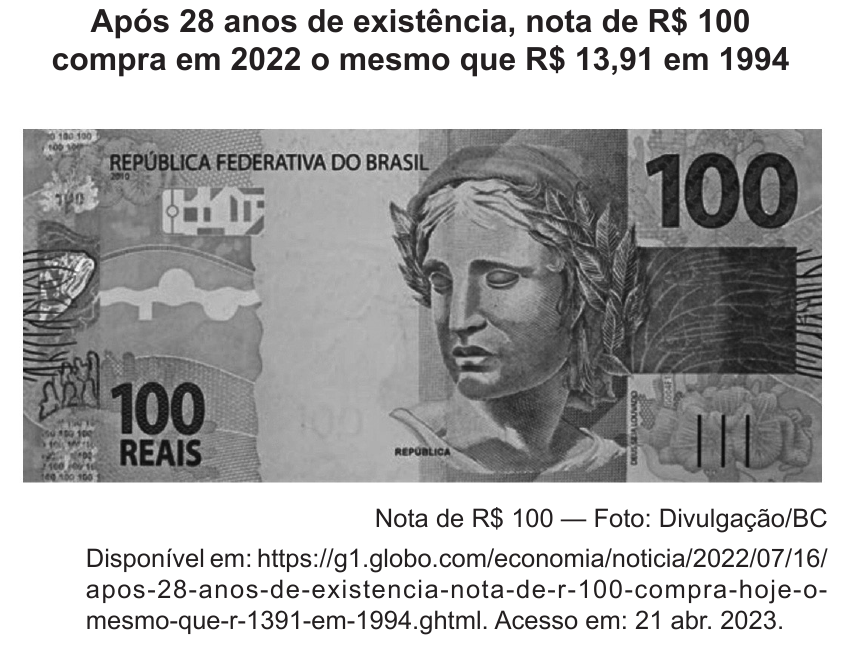
\includegraphics[scale=.5]{fig003.png}\\Suponha que, em 1994, um artigo custasse R\$ 13,91 e,
exatos 28 anos depois (336 meses), ele passasse a custar R\$ 100,00. Suponha, também, que, para esse período, a taxa mensal de aumento no preço desse artigo tenha sido igual a k\%, ou seja, a cada mês o preço do artigo sofreu um aumento de k\% em relação ao preço do mês anterior. O valor de k pode ser dado por}{
\item $100 \left(\dfrac{100}{13,91}\right)^{1/336}-100$
\item $100 \left(\dfrac{100}{13,91}\right)^{336}-100$
\item $\left(\dfrac{100}{13,91}\right)^{1/336}-1$
\item $\left(\dfrac{100}{13,91}\right)^{336}+0,01$
\item $100 \left(\dfrac{100}{13,91}\right)^{1/336}+0,01$
}{https://youtu.be/fDPDxc8zjzY}
\chapter{Operações Básicas}

\quest{Técnico Interno BBTS 2023 - FGV}{Um joalheiro fabrica correntes de ouro, todas iguais. Para cada quilograma de ouro que recebe, ele o divide em 50 partes iguais e fabrica uma corrente usando 3 dessas partes. Certo dia, o joalheiro recebeu 900g de ouro.
Assinale a opção que indica o número de correntes que ele conseguiu fabricar com essa quantidade de ouro.}{
\item 10.
\item 12.
\item 15.
\item 18.
\item 20.}
{https://youtu.be/bR6l1KD3z94}

\quest{Guarda Metropolitano Prefeitura de Palmas TO - VUNESP 2023}
{Ao longo de uma avenida foram colocados tapumes de proteção para a execução de uma obra. Ao todo foram colocados 90 tapumes, seguindo sempre o seguinte padrão de cores: 5 tapumes brancos seguidos de um tapume laranja. Nessas condições, e sabendo que o primeiro tapume colocado era branco, o número total de tapumes laranja colocados foi}{
\item 12.
\item 15.
\item 18.
\item 21.}
{https://youtu.be/vYrGL-V7HWE}
\chapter{Porcentagens}

\quest{Técnico Administrativo - IBFC 2023}{
Paulo foi a uma loja e pagou R\$ 238,00 por um produto, já incluso 15\% de desconto sobre o
preço do produto exposto na vitrine. Nessas condições, o valor do desconto atribuído ao preço do produto foi de:}{
\item R\$ 42,00
\item R\$ 35,70
\item R\$ 36,00
\item R\$ 48,00}
{https://youtu.be/FMTZR0kfBjk}

\quest{Guarda Metropolitano Prefeitura de Palmas TO - VUNESP 2023}{O segurança de uma empresa trabalha em turnos de 6 horas por noite e faz rondas no prédio inteiro, gastando em cada ronda 13 minutos e 30 segundos. Sabendo que esse segurança faz 4 rondas durante o seu turno e supondo que ele mantenha sempre o mesmo tempo por ronda, então, em relação ao turno de 6 horas, o tempo total gasto nessas 4 rondas corresponde a}{
\item 15\%.
\item 20\%.
\item 25\%.
\item 30\%.}
{https://youtu.be/jrBTcWimYvM}

\quest{Guarda Metropolitano Prefeitura de Palmas TO - VUNESP 2023}{Participaram de um concurso público 1200 candidatos, dos quais 30\% foram aprovados. Entre os aprovados, alguns foram chamados imediatamente, e os demais ficaram na lista de espera. Se a razão do número de candidatos chamados imediatamente para o número de candidatos que ficaram na lista de espera foi $\dfrac{2}{3}$, o número de candidatos que ficaram na lista de espera foi}{
\item 162.
\item 180.
\item 198.
\item 216.}
{https://youtu.be/YPlaAEBhOfA}
\chapter{Potenciação e Radiciação}

\section{Potenciação}
\quest{Transpetro 2023 - CESGRANRIO}{Considerando-se os números reais $2^{75}$, $3^{50}$ e $4^{37}$, o menor e o maior deles são, respectivamente,
}{
\item $4^{37}$ e $3^{50}$
\item $4^{37}$ e $2^{75}$
\item $3^{50}$ e $2^{75}$
\item $3^{50}$ e $4^{37}$
\item $2^{75}$ e $4^{37}$
}{https://youtu.be/qZ4qR2DjaIE}

\quest{Transpetro 2023 - CESRANRIO}
{O quadrado de um número real $x$ é representado por $x^2$, e é definido por $x^2 = x \cdot x$. A condição $x \leqslant x^2$ é FALSA quando $x$ é igual a}
{
\item 0
\item $\dfrac{1}{2}$
\item 1
\item $-\dfrac{1}{2}$
\item $\dfrac{3}{2}$
}{https://youtu.be/1hJNHbCNVUc}

\chapter{Probabilidades}

\quest{Técnico Administrativo - IBFC 2023}{Ana esqueceu a senha de seu cartão de crédito. Ela só lembra que ela é formada por 4 letras
maiúsculas sem repetição (todas vogais) e que a primeira vogal é a letra E. Desse modo, a probabilidade de Ana acertar sua senha do cartão de crédito numa única tentativa é igual a:}
{
\item $\dfrac{1}{125}$
\item $\dfrac{1}{3}$
\item $\dfrac{1}{24}$
\item $\dfrac{1}{4}$}
{https://youtu.be/CMn8ztjOdR8}

\quest{Técnico Interno BBTS 2023 - FGV}{Um dado cúbico honesto com as faces numeradas de 1 a 6 é lançado 3 vezes consecutivas. Sabe-se que o número sorteado no primeiro lançamento é a soma dos números sorteados nos outros dois lançamentos. A probabilidade de o número 1 (um) ter sido sorteado pelo menos uma vez é}{
\item $ \dfrac{1}{6}.$
\item $ \dfrac{1}{3}.$
\item $ \dfrac{2}{3}.$
\item $ \dfrac{2}{5}.$
\item $ \dfrac{3}{5}.$}
{https://youtu.be/OgFUUsHP4hU}
\chapter{Razão e Proporção}
\quest{Oficial de Justiça 2023 - VUNESP}{No ano de 2022, 3 em cada 8 edifícios comercializados em determinada região foram adquiridos pelo empreendimento A&B, que investiu R\$ 1,35 bilhão na compra desses edifícios, ao preço médio de R\$ 15 milhões cada edifício. Dos edifícios não adquiridos pelo empreendimento A&B e que foram comercializados naquela r­egião, o empreendimento R&T adquiriu metade, ao custo total R\$ 1,23 bilhão, o que fez com que o preço médio, por edifício adquirido pela R&T, fosse de}
{
\item R\$ 16,3 milhões.
\item R\$ 16,1 milhões.
\item R\$ 16,5 milhões.
\item R\$ 16,4 milhões.
\item R\$ 16,2 milhões.}
{https://youtu.be/41SHCi5jX54} 

\quest{Técnico Interno BBTS 2023 - FGV}{Oscar, na primeira metade de uma partida de basquete, acertou 12 de 16 arremessos e, na segunda metade, acertou os 8 arremessos que fez. Jordan, por sua vez, fez 12 arremessos na primeira metade do jogo e 18 arremessos na segunda metade. Em cada metade do jogo, o percentual de acertos de Oscar foi maior do que o percentual de acertos de Jordan. Entretanto, ao final do jogo, os percentuais de acerto totais dos dois jogadores foi o mesmo. Na segunda metade do jogo, o número de acertos que Jordan teve a mais do que o seu número de acertos na primeira metade foi}{
\item 9.
\item 10.
\item 11.
\item 12.
\item 13.}
{https://youtu.be/jgkJfktwl98}

\chapter{Regra de Três Simples e Composta}

\quest{Oficial de Justiça 2023 - VUNESP}
{Considere as informações apresentadas na tabela a seguir, relacionadas à produção de certa peça que é
realizada apenas por máquinas iguais, trabalhando ao mesmo tempo, com a mesma capacidade de produção.\\
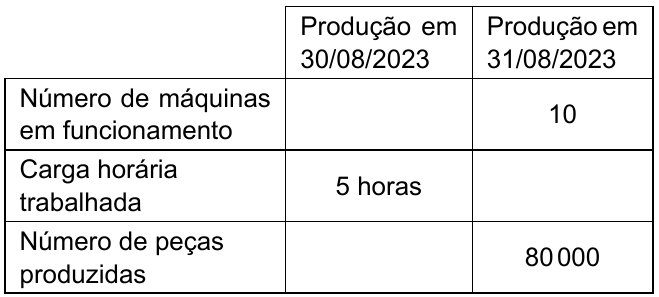
\includegraphics[scale=.5]{fig002.png}\\
Sabendo-se que as informações apresentadas são proporcionais, que em 30/08/2023 o número de máquinas
em funcionamento era um quinto maior que o número de máquinas trabalhando no dia seguinte, e que o número
de peças produzidas em 31/08/2023 foi quatro terços do número de peças produzidas no dia anterior, é correto afirmar que a carga horária trabalhada no dia 31/08/2023 foi de}
{\item 8 horas.
\item 7 horas.
\item 9 horas.
\item 8 horas e 30 minutos.
\item 7 horas e 30 minutos.}
{https://youtu.be/mVp0Bf8s8J4}

\chapter{Sequências}
\quest{Oficial de Justiça 2023 - VUNESP}{ Na sequência numérica 1, 4, 7, 8, 11,14, 19, 22, 25, 26, 29, 32, 37, ..., o 1º elemento é o número 1. Mantida a regularidade, o 11 111º elemento é o número}
{ 
\item 33 332.
\item 31 111.
\item 33 115.
\item 33 329.
\item 32 228.
}{https://youtu.be/whv3ZbhWa9U}
\chapter{Sistemas de Equações}

\quest{Transpetro 2023 - CESGRANRIO}{Em um torneio de videogame, o menino J disputou apenas três partidas, fazendo um total de 2.660 pontos. Na segunda partida, ele fez 410 pontos a mais do que fez na primeira; na terceira partida, fez apenas metade de pontos que fez na segunda. O número de pontos feitos por J, apenas na primeira partida, quando dividido por 5, deixa resto igual a}
{
\item 4
\item 3
\item 2
\item 1
\item 0}
{https://youtu.be/F8m70a4IGRs}

\quest{Transpetro 2023 - CESGRANRIO}{Um consumidor foi ao mercado, comprou 1 kg de batata e 1 kg de cebola e pagou R\$ 11,00. No dia seguinte,
ele comprou 3 kg de batata e 2 kg de cebola e pagou R\$ 28,00. No terceiro dia, ele comprou 2 kg de batata e 1 kg de cebola.\\
Considerando-se que os preços não foram alterados durante esse período, que valor, em R\$, o consumidor pagou no terceiro dia?}
{
\item 5
\item 6
\item 16
\item 17
\item 39}
{https://youtu.be/IQyQnHNrd7g}
\chapter{Sistemas de Medidas}

\section{Medidas de Tempo}

\quest{Transpetro 2023 - CESGRANRIO}
{Um carro partiu de um ponto A até um ponto B andando com uma velocidade constante de 80 km/h. Posteriormente o carro refez o mesmo percurso, mas agora com velocidade constante igual a 100 km/h, e gastou 30 minutos a menos do que na primeira vez. Quanto tempo o carro levou para ir do ponto A ao ponto B, na primeira vez?}
{
\item 3h
\item 2h30min
\item 2h
\item 1h50min
\item 1h30min
}
{https://youtu.be/XsGBfA6alQ4}
\chapter{Raciocínio Lógico}

\quest{Oficial de Justiça 2023 - VUNESP}{ Sabendo-se que é falsidade a afirmação “Se Nora trabalhou, então ela precisa descansar”, assinale a alternativa que apresenta uma afirmação verdadeira.}{
\item Nora trabalhou e ela não precisa descansar.
\item Nora não trabalhou e ela não precisa descansar.
\item Nora trabalhou e ela precisa descansar.
\item Nora não trabalhou ou ela precisa descansar.
\item Nora não trabalhou e ela precisa descansar.}{https://youtu.be/DQVfJCeKXF8}

\quest{Oficial de Justiça 2023 - VUNESP}
{Considere verdadeiras as seguintes premissas:
\begin{enumerate}[I.]
\item Se Carla não é casada ou Pedro não é divorciado, então Cláudio é filho único.
\item Se Sônia é mãe, então Carla não é casada.
\item Se Pedro não é divorciado, então Sergio não é administrador e Gerson é noivo.
\item Cláudio não é filho único.
\end{enumerate}
Uma conclusão que decorre das premissas apresentadas
e forma, juntamente com as premissas, um argumento
válido é
}{\item Gerson é noivo.
\item Sergio não é administrador.
\item Sônia não é mãe.
\item Sônia é mãe.
\item Sergio é administrador.}
{https://youtu.be/XXmDn4BTLn8}

\quest{Oficial de Justiça 2023 - VUNESP}
{Considere a seguinte afirmação: “Ou durmo ou trabalho”.
Uma negação lógica para a afirmação apresentada é}{
\item Ou não durmo ou não trabalho.
\item Trabalho ou durmo.
\item Se não durmo, então não trabalho.
\item Não trabalho e não durmo.
\item Durmo se, e somente se, trabalho.}
{https://youtu.be/w22pO_WZ_dk}

\quest{Oficial de Justiça 2023 - VUNESP}
{Considere verdadeira a afirmação “Se Marcelo é professor universitário, então Raquel é advogada” e falsa a afirmação “Marcelo é professor universitário e Raquel é advogada”. Nessas condições, é necessariamente verdade que}{
\item Marcelo não é professor universitário.
\item Raquel não é advogada.
\item Marcelo é professor universitário.
\item Marcelo é professor universitário ou Raquel não é advogada.
\item Raquel é advogada.}
{https://youtu.be/kQjrUqqL9eM}

\quest{Técnico Administrativo - IBFC 2023}{ Se todo vegetal é nutritivo e alguns alimentos
são nutritivos, então é correto afirmar que:}{
\item Todo alimento é vegetal
\item Não pode haver alimento que é vegetal
\item Não pode haver alimento que não é vegetal
\item Pode haver vegetal que não é alimento}
{https://youtu.be/ka6Kcb0-Vf8}

\quest{Técnico Administrativo - IBFC 2023}{Se o valor lógico de uma proposição p é verdade e o valor lógico de uma proposição q é falso, então é correto afirmar que:}{
\item A conjunção entre p e q tem valor lógico verdade
\item O bicondicional entre p e q tem valor lógico falso
\item A disjunção entre p e q tem valor lógico falso
\item A disjunção exclusiva entre p e q tem valor lógico falso}
{https://youtu.be/vkQIpeSXZCY}

\quest{Técnico Interno BBTS 2023 - FGV}{Considere a afirmação a seguir.
“Eu fiz dieta e não emagreci.”\\
A negação lógica dessa afirmação é:}{
\item Eu não fiz dieta e não emagreci.
\item Eu não fiz dieta ou emagreci.
\item Eu não fiz dieta e emagreci.
\item Eu não fiz dieta ou não emagreci.
\item Eu fiz dieta e emagreci.}
{https://youtu.be/16Po-EIt1ec}
\chapter{Raciocínio Lógico Matemático}

\quest{Técnico Interno BBTS 2023 - FGV}
{Uma caixa A tem 10 bolas azuis e, uma caixa B, 10 bolas verdes. Foram transferidas 7 bolas da caixa A para a caixa B e, a seguir, aleatoriamente, 5 bolas da caixa B para a caixa A. É correto concluir que, ao final,}{
\item a caixa A tem mais bolas azuis do que a B.
\item a caixa B tem mais bolas verdes do que a A.
\item a caixa A tem, no máximo, 6 bolas azuis a mais do que a B.
\item a caixa B tem, no mínimo, 2 bolas azuis a mais do que a A.
\item as duas caixas têm o mesmo número de bolas verdes.}
{https://youtu.be/DEqIJTPZjEY}
\chapter{Verdades e Mentiras}
\quest{Banco do Brasil 2023 - CESGRANRIO}{As irmãs N, T e S apostaram uma corrida. Elas têm uma
peculiaridade: N nunca mente; T às vezes mente; S sem-
pre mente.
\begin{itemize}
\item Quem ficou em 1º lugar disse: “S ficou em 2º lugar”.
\item Quem ficou em 2º lugar disse: “Eu sou T”.
\item Quem ficou em 3º lugar disse: “N ficou em 2º lugar”.
\end{itemize}
Nessa corrida, tem-se como 1º lugar, 2º lugar e 3º lugar, respectivamente,}
{
\item S, T, N
\item T, S, N
\item N, T, S
\item T, N, S
\item N, S, T}
{https://youtu.be/cpwaA8oIobw}
\end{enumerate}




\end{document}